%!TEX root = ../main.tex

\graphicspath{{../Pictures/04_construccion/}, % Carpeta capitulo
              {../Pictures/}                  % Carpeta general
              }

\begin{document}
%=================================================================
%                           Start Document
%=================================================================
% Carpeta imagenes capitulo
% \graphicspath{{Pictures/04_construccion/},{Pictures}}


\chapterimage{marmol.pdf}

\chapter{Fantoma de mama para tratamientos por medio de hipertermia}

\section{Construcción del fantoma}

\subsection{Introducción}\index{Introducción}

Un fantoma es toda construcción tangible-material o teórica-matemática, que se emplea especialmente en el área de la física médica con la finalidad de evaluar el comportamiento que esta estructura presenta al interactuar con una determinada forma de energía, dentro de sus usos destacan el de ser el modelo para el diseño de equipos médicos o ser el medio por el cual se realiza la calibración y control de los rangos de operación de los mismos equipos. Por otra parte, un material mimético MM es todo aquel creado de forma artificial mediante procesos químicos que busca imitar las propiedades de uno o varios materiales naturales o artificiales, muchas veces con la idea de reducir costes, evitar tener que exponer materiales In-vivo o Ex-vivo e incluso potencializar ciertas características del material como por ejemplo su durabilidad o características de interés al momento de realizar pruebas de campo, por ejemplo sus propiedades dieléctricas como la conductividad, la permitividad, sus propiedades acústicas como la velocidad del sonido, atenuación, propiedades mecánicas entre las que destacan el módulo de Young, etc \cite{A007:farrer2015characterization} \cite{A019:lazebnik2005tissue}.  

\subsection{Justificación}\index{Justificación}

Los materiales basados en gelatina son atractivos debido a sus propiedades mecánicas estables y facilidad de fabricación, en trabajos anteriores se han descrito recetas basadas en agua y gelatina que permiten simular tejidos con alto contenido de agua en un rango de frecuencias comprendido entre los 10 y los 50 $MHz$, además de que era posible construir muestras con un amplio rango de propiedades dieléctricas simplemente con variar la concentración de gelatina, sin embargo, estas muestras no eran apropiadas para la elaboración de fantomas homogéneos debido a la difusión de soluto o solvente existente cuando dos materiales con distintas concentraciones de gelatina son puestos en contacto, por ende con el paso del tiempo las propiedades dieléctricas obtenidas inicialmente tendían a variar. Otra dificultad radica en que la mayoría de materiales simulan las propiedades dieléctricas en un ancho de banda estrecho para el cual fueron diseñados, lo que hace que la composición de los materiales deba cambiar para cada frecuencia de interés \cite{A019:lazebnik2005tissue}. \\ 

Debido a que el seno es un volumen de tejido heterogéneo con estructuras constitutivas que poseen propiedades dieléctricas que abarcan todo el espectro biológico, por ejemplo MM para tejidos con bajo contenido de agua (tejido adiposo), para tejidos con alto contenido de agua (tejido glandular y canceroso) y tejidos con contenido intermedio de agua (piel), vale la pena recalcar la necesidad de construir fantomas estables y antropomórficos que puedan tener una composición heterogénea al yuxtaponer muchos MM sin el riesgo de que sus propiedades cambien debido a difusión a través de las interfaces y que a su vez funcione para un ancho de banda amplio \cite{A019:lazebnik2005tissue}. \\ 

Lazebnik propone y caracteriza dispersiones de aceite en gelatina que da como resultado un MM con características que se aproximan a las propiedades dieléctricas de una gran variedad de tejidos humanos en un rango de microondas comprendido entre los 500 $MHz$ y los 20 $GHz$, en este basta con el cambio de la concentración de aceite para modificar las propiedades del MM de acuerdo al tejido que se desea mimetizar, además de que su estructura se mantiene estable por largos periodos de tiempo, 9 semanas aproximadamente para las pruebas que realizaron, donde los cambios en la geometría y en las propiedades dieléctricas fue despreciable \cite{A019:lazebnik2005tissue}. \\ 

A continuacion se presentan los pasos necesarios para la construccion del fantoma, para obtener las medidas de los materiales empleados en la construccion del mismo se debe revisar la tabla \ref{tab:porcentajePesoIngredientes} de acuerdo al tejido que se desee emular

\begin{table}[H]
 \centering \caption{Porcentaje por peso de los distintos ingredientes necesarios para la elaboración de los fantomas de distintas estructuras anatómicas con distintas concentraciones de aceite. Abreviaturas: Filas: V.acte - Volumen de aceite, Fibgln - Tejido Fibroglandular.  Columnas: Surf - Surfactante, A.Benz - Acido Benzoico, Prpgcl - Propilenglicol.}
 \label{tab:porcentajePesoIngredientes}
\begin{tabular}{lcccc}
\hline
	     & Tumor	&	Piel	&	Fibgln &	Grasa	\\
\hline
\hline
V.acte  &	10 \%	&	20 \%	&	50 \%	 &	80 \%	\\
\hline
Aceite  &	7.57	&	17.17	&	41.05	 &	62.03	\\
Agua    &	73.59	&	66.65	&	39.70	 &	14.20	\\
Surf 	  &	2.18	&	1.10	&	10.27	 &	13.11	\\
Formol  &	0.31	&	0.28	&	0.17	 &	0.06	\\
A. Benz &	0.08	&	0.07	&	0.04	 &	0.02	\\
Prpgcl 	&	3.10	&	2.80	&	1.67	 &	0.74	\\
Gelatin &	13.17	&	11.93	&	7.11	 &	9.84	\\
\hline
\end{tabular}
\end{table}

\subsection{Construcción}\index{Construcción}

\begin{enumerate}

\item Haciendo uso de una luna de reloj y la balanza de laboratorio mida la cantidad indicada de Acido Benzoico.

\item Haciendo uso de una pipeta con bulbo tome la cantidad indicada de formol y viértala en un baker.

\item Añada el ácido benzoico en el baker donde se encuentra contenido el formol, caliente el baker en una placa calefactora hasta alcanzar los 90 \degree C, esto con la finalidad de que el ácido benzoico se disuelva. Debido a que las cantidades usadas son muy pequeñas, es recomendable preparar una cantidad mayor a la empleada en el fantoma y almacenar el producto resultante en un recipiente sellado para luego usarlo de acuerdo a los requerimientos del mismo. Figura \ref{fig:01mezclaFormolAcido}.

    \begin{figure}[H]
    \centering
    \begin{minipage}{0.45\textwidth}
        \centering
        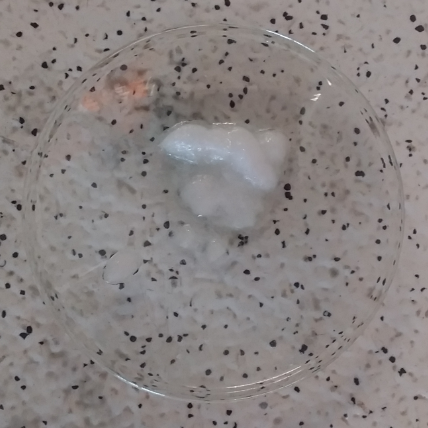
\includegraphics[width=6cm, keepaspectratio]{01mezclaFormolAcido.png} 
        \caption{Muestra de la mezcla formol ácido benzoico en la luna de reloj.}
        \label{fig:01mezclaFormolAcido}
    \end{minipage}\hfill
    \begin{minipage}{0.45\textwidth}
        \centering
        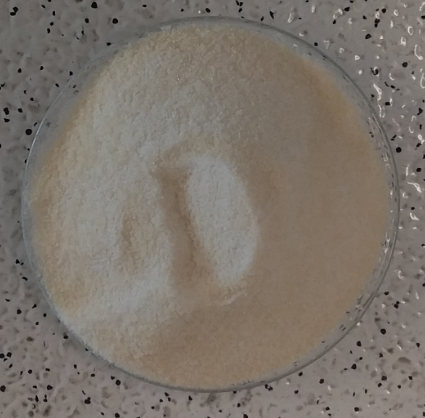
\includegraphics[width=6cm, keepaspectratio]{02Gelatina.png}
        \caption{Muestra de gelatina en la luna de reloj.}
        \label{fig:02Gelatina}
    \end{minipage}
    \end{figure}

\item Haciendo uso de una luna de reloj y una balanza de laboratorio mida la cantidad indicada de gelatina, luego viértala en un sartén. Figura \ref{fig:02Gelatina}.

\item Haciendo uso de una probeta milimetrada mida la cantidad indicada de agua desionizada y viértala en el sartén donde se encuentra la gelatina, mezcle la gelatina con el agua esto con la finalidad de hidratarla.

\item Vierta la mezcla Formol-Acido Benzoico en el sartén y mezcle.

\item Haciendo uso de una pipeta con bulbo tome la cantidad indicada de propilenglicol, viértala en el sartén y mezcle. Figura \ref{fig:03Propilenglicol}.

\item Caliente el sartén en la placa calefactora mezclando continuamente el contenido de la misma hasta alcanzar los 55 \degree C temperatura a la cual se funde la gelatina. Figura \ref{fig:04calentarMezcla}.

\item En un Baker mida la cantidad indicada de aceite de oliva, luego tome el Baker y haciendo uso de una placa calefactora caliente su contenido hasta alcanzar los 50 \degree C. Figura \ref{fig:05calentarAceite}.

\item Vierta el contenido del sarten en el Baker que contiene el aceite.

    \begin{figure}[H]
    \centering
    \begin{minipage}{0.45\textwidth}
        \centering
        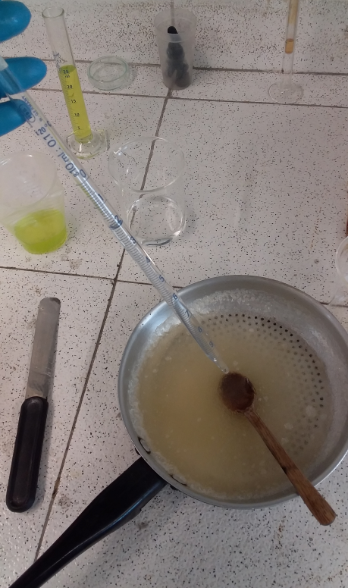
\includegraphics[width=4cm, height=6.8cm]{03Propilenglicol.png}
        \caption{Adición del propilenglicol a la mezcla por medio de la pipeta.}
        \label{fig:03Propilenglicol}
    \end{minipage}\hfill
    \begin{minipage}{0.45\textwidth}
        \centering
        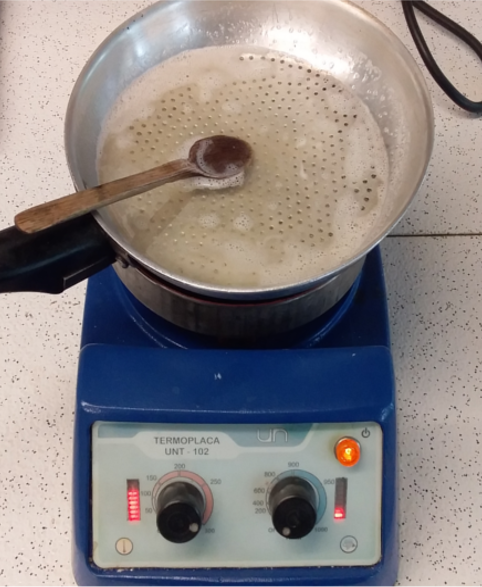
\includegraphics[height=6.8cm, keepaspectratio]{04calentarMezcla.png}
        \caption{Calentamiento de la mezcla hasta alcanzar el punto de fusión de la gelatina.}
        \label{fig:04calentarMezcla}
    \end{minipage}
    \end{figure}

\item Haciendo uso de una probeta mida la cantidad indicada de surfactante y agréguela en la mezcla aceite-gelatina, el color de la mezcla se tornara amarillo blanquecino. Figura \ref{fig:06mezclaSurfactante}. 

\item Permita que la mezcla se enfríe hasta alcanzar los 34 \degree C para poder verterla en los moldes.

    \begin{figure}[H]
    \centering
    \begin{minipage}{0.45\textwidth}
        \centering
        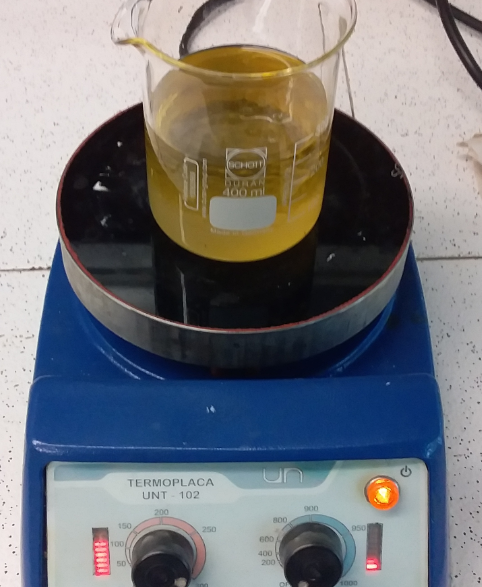
\includegraphics[height=6.8cm, keepaspectratio]{05calentarAceite.png}
        \caption{Baker con aceite sobre la placa calefactora.}
        \label{fig:05calentarAceite}
    \end{minipage}\hfill
    \begin{minipage}{0.45\textwidth}
        \centering
        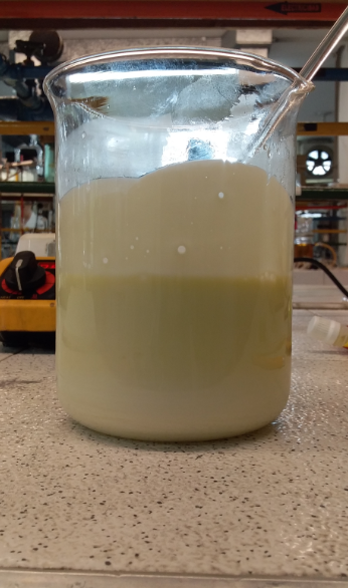
\includegraphics[width=4cm, height=6.8cm]{06mezclaSurfactante.png}
        \caption{Color amarillo blanquecino adquirido por la mezcla aceite-gelatina al agregar el surfactante.}
        \label{fig:06mezclaSurfactante}
    \end{minipage}
    \end{figure}

\end{enumerate}

Es recomendable mantener cubiertas las zonas expuestas del molde o incluso el fantoma cuando se encuentre desmoldado, haciendo uso de alguna película plástica que se encuentre en contacto con la superficie del fantoma, esto con el fin de evitar la desecación del mismo.

\textbf{Nota:}
La desecación es el proceso de formación de grietas poligonales en el fantoma al perder humedad, otra consecuencia de la perdida de humedad es la sedimentación donde las partículas en suspensión, en este caso aceite, tienden a asentarse y acumularse en la parte inferior del sistema, esto se debe a su diferencia de densidades, su insolubilidad y a la respuesta a fuerzas externas que actúan sobre el sistema, por ejemplo la gravedad.

\section{Simulación}

Meshmixer es un programa diseñado para trabajar con mallas de triangulos tridimensionales, dichas mallas son una colección de triangulos y vertices que se aproximan una superficie 3D, dichas superficies pueden ser obtenidas por medio del uso de escaneres, lo cual es muy útil en aplicaciones médicas, debido a que los doctores pueden escanear una persona, generar un modelo 3D especifico del paciente y luego hacer uso del mismo para crear dispositivos y ayudas personalizados.

Un ejemplo de ello es el trabajo del Dr Ciprian Ionita y su equipo \cite{ A029:kurenov2015three}


    \begin{figure}[H]
    \centering
    %-----------------------------------
    \begin{subfigure}[t]{0.45\textwidth}
        \centering
         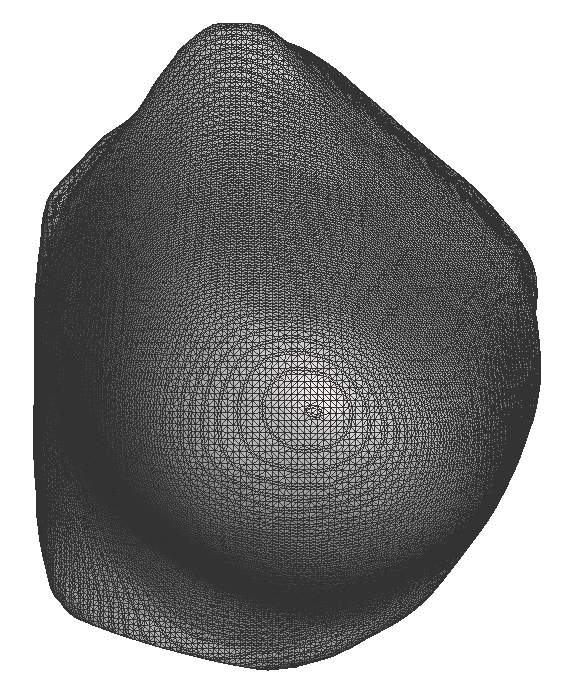
\includegraphics[width=7cm, keepaspectratio]{04_construccion/breast-scanned.png}
        %\caption{Mirror 1 movement direction, considering the position that the DMD will have.}
        %\label{img:Paso2B}
    \end{subfigure}
    %-----------------------------------
    \begin{subfigure}[t]{0.45\textwidth}
        \centering
        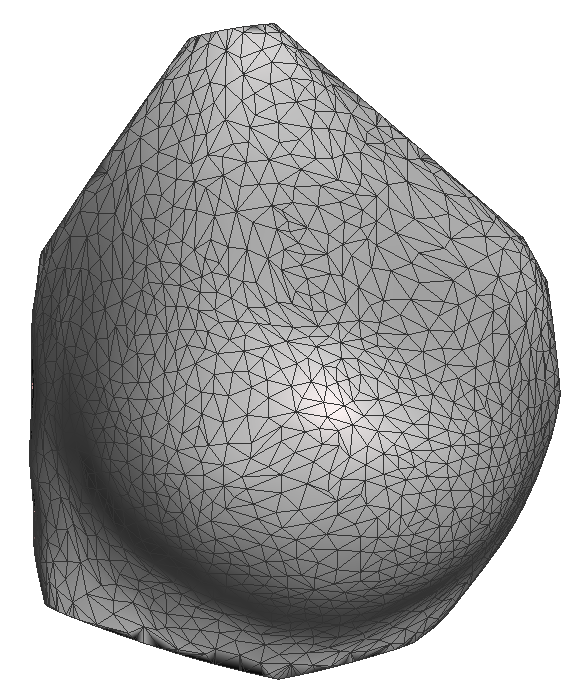
\includegraphics[width=7cm, keepaspectratio]{04_construccion/breast-clean.png}
        %\caption{The mirror must be perpendicular to the plane of incidence of the beam.}
        %\label{img:Paso2A}
    \end{subfigure} 
    %-----------------------------------
    %\caption{Graphical description of step 2.}
    %\label{img:BMS-corrected}
    \end{figure}

La tasa de absorción específica, comúnmente conocida en inglés como SAR (Specific Absorption Rate), es la unidad de medida empleada para medir la cantidad de energía que es absorbida por un cuerpo al ser expuesto a un campo electromagnético de radiofrecuencia, de acuerdo con Chou \cite{A028:chou1996radio}, la SAR es determinada no solo por las ondas electromagnéticas incidentes sino también por las características eléctricas y geométricas tanto del cuerpo expuesto a la radiación como de los objetos cercanos.

\begin{equation}
    SAR = SAR = \frac{d}{dt} \bigg( \frac{\partial W}{\partial m} \bigg)
\end{equation}

\begin{equation}
    SAR = SAR = \frac{d}{dt} \bigg( \frac{\partial W}{\rho \cdot \partial V} \bigg)
\end{equation}

\begin{equation}
    PLD = \frac{d}{dt} \bigg( \frac{\partial W}{\partial V} \bigg)
\end{equation}

%==============================================================
%                           End Document
%==============================================================
\end{document}